\begin{frame}{Background -- Elementary Functions}
    \pause \vspace{-2em}
    \begin{minipage}[t]{0.48\linewidth}
        \begin{definition}[%Elementary functions,
                           \citep{OrdinaryDifferentialEquations_Morris_Tenenbaum_1985}]
            The \textbf{elementary functions} on $\Reals$  are partial functions defined by expressions built up from 
            \pause

            \kern-1ex
            \begin{itemize}
                \setlength\itemsep{-1pt}
                \item computable reals, and
                \item the variable $x$,
            \end{itemize}
            \kern-1ex
            \pause by applying (repeatedly) the basic operations below on elementary functions $f,g$:
            \pause
            \begin{itemize}
                \setlength\itemsep{-1pt}
                \item $(f+g)(x) = f(x) + g(x)$ 
                \item $(f\cdot g)(x) = f(x)g(x)$
                \item $\mathrm{div}_f(x) = \frac{1}{f(x)}$ \kern5em where $\frac{1}{0} =\ \uparrow$
                \item $\mathrm{root}_{n,f}(x) = \sqrt[n]{f(x)}$ \hfill where $0< n \in \Nats$
                \item $\ln_f(x) = \ln(f(x))$
                \item $\exp_f(x) = e^{f(x)}$
                \item $\sin_f(x) = \sin(f(x))$
                \item $\arcsin_f(x) = \arcsin(f(x))$
            \end{itemize}
        \end{definition}
    \end{minipage}
    \hfill
    \pause \begin{minipage}[t]{0.45\linewidth}
        \begin{exampleblock}{\textbf{\textcolor{BrickRed}{Problem}}}
            The domains of elementary functions are not all open!
        \end{exampleblock}
        \pause
        \begin{exampleblock}{\color{OliveGreen}\textbf{Solution: Modifications}}
            \pause
            \begin{itemize}
                \item We define $\sqrt[n]{x} = 0$ for $x < 0$ when $n$ is even.
                \pause \item We extend the definition of $\arcsin(x)$ to be $\frac{\pi}{2}$ for $x > 1$ and to be $-\frac{\pi}{2}$ for $x<-1$.
            \end{itemize}
        \end{exampleblock}
        \centering
        \visible<7->{
        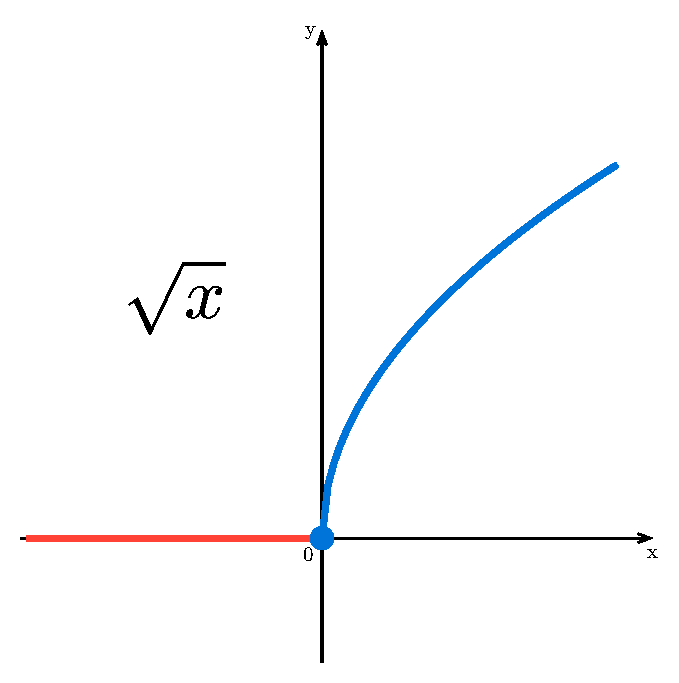
\includegraphics[width=0.35\linewidth]{sqrt.pdf}
        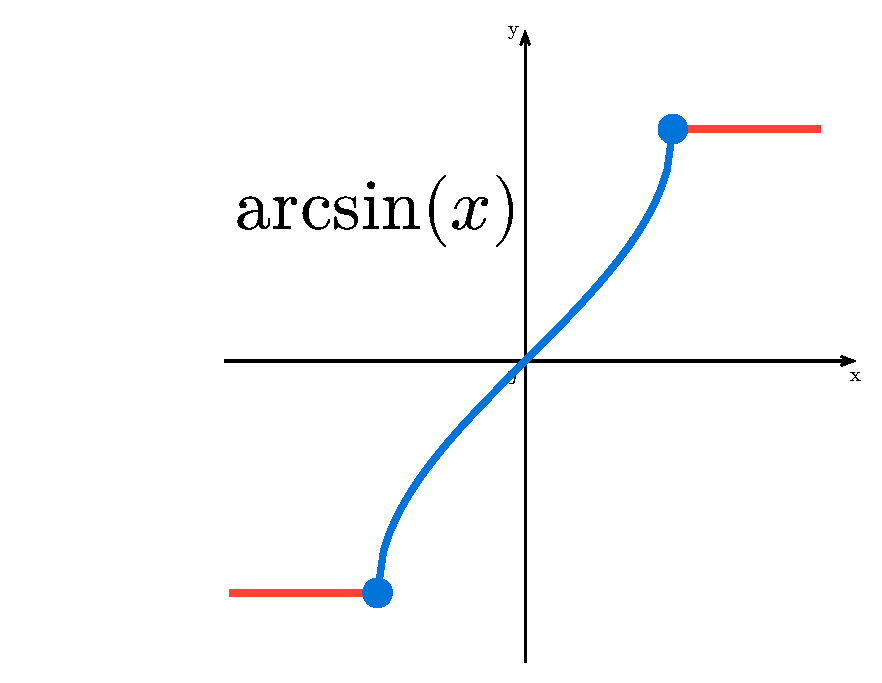
\includegraphics[width=0.35\linewidth]{arcsin.pdf}}
    \end{minipage}\kern-0.2em
    \note[item]{So the idea of the solution was to prove acceptability of elementary functions. Now that we have the definition of acceptability, we also need to review the definition of elementary functions.}
    \note[item]{
    Elementary functions are unary functions on $\Reals$, built up from the variable $x$ and compuatble reals, field operations, $n$th root, logarithm, exponential, and trigonometric functions. Note that addition and multiplication here are still unary functions.}
    \note[item]{Can we prove acceptability of elementary functions in their current forms? Looking more closely, we can see that not all the domains of the functions we just defined are open. So they cannot have effective open exhaustions for their domains.}
    \note[item]{What we can do to solve this, is to modify these functions to have open domains. Specifically we define even roots of a negative number to be $0$ and $\arcsin(x)$ to be defined as $\pi/2$ for $x>1$ and $-\pi/2$ for $x<-1$.}
\end{frame}